\documentclass[12pt]{article}
\usepackage[hmargin=1in,vmargin=1in]{geometry}
\usepackage{amsmath}
\usepackage{setspace}
\usepackage{graphicx}
\usepackage{sectsty}
\usepackage{fancyvrb}
\usepackage{mathtools}
\usepackage{float}
\usepackage[flushleft]{threeparttable}

% Make all of the environments for different proof elements
\newtheorem{theorem}{Theorem}[section]
\newtheorem{lemma}[theorem]{Lemma}
\newtheorem{proposition}[theorem]{Proposition}
\newtheorem{corollary}[theorem]{Corollary}
\newenvironment{proof}[1][Proof:]{\begin{trivlist}
\item[\hskip \labelsep {\bfseries #1}]}{\end{trivlist}}
\newenvironment{definition}[1][Definition]{\begin{trivlist}
\item[\hskip \labelsep {\bfseries #1}]}{\end{trivlist}}
\newenvironment{example}[1][Example]{\begin{trivlist}
\item[\hskip \labelsep {\bfseries #1}]}{\end{trivlist}}
\usepackage{hyperref}
\usepackage[usenames, dvipsnames]{color}

\definecolor{cuse}{RGB}{212, 69, 0}
\definecolor{uva}{RGB}{0, 55, 119}

% Change back to use Arabic footnotes
\renewcommand*{\thefootnote}{\arabic{footnote}}
\sectionfont{\large}
\subsectionfont{\normalsize}

% Start the document
\begin{document}
\setcounter{page}{1}
\begin{doublespacing}

\title{Draft Empirics Section}
\author{David Freed and Samuel Green}
\date{April 30, 2016}
\maketitle

This section lays out support for the theoretical hypotheses presented earlier. Section 4.1 demonstrates that Twitter is responsive to large swings in the game and can effectively incorporate information about game events. Section 4.2 demonstrates that both Twitter volume and aggregate Twitter sentiment can predict future events in the game. After showing the predictive power of our variables, we conclude in Section 4.3 by demonstrating that they constitute an improvement on prior models. We compare standard logistic regression models with those incorporating Twitter information, showing the latter is more predictive of the final outcome at each point in the game. 

\section*{Twitter's Ability to Process Prior Events}

The first idea that we want to assess is whether Twitter is able to process game events as they happen. As discussed in the previous section, we use a modified uniform approximation to map game times to real times, allowing us to capture subsets of Tweets that occurred in the time surrounding an event. To empirically test this result, we divided up our dataset for each game into a series of one-minute intervals. For each interval, we not only measured the change in margin (i.e. how Team 1's lead/deficit changed over the course of the minute) but also the change in Twitter sentiment and change in Twitter volume for both teams. 

If Twitter is responsive to events in the game, then Twitter sentiment and volume for a given team should spike as their play improves. We have already seen evidence of this in previous figures, which showed that Tweet sentiment and volume about Syracuse increased drastically as they made their comeback against Virginia. Over the same time, sentiment and volume plateaued for the Cavaliers. 

In Table \ref{table:sentresponsiveness}, we look at whether the difference in margin\footnote{We define margin in period $t$ as the difference between the number of points scored by Team 1 in period $t$ and the number of points scored by Team 2 in period $t$.} in period $t-1 $ can predict the sentiment difference in period $t$. The variable \texttt{Margin\_Period\_Lag\_1} represents the change in the lead/deficit in the prior period, while \texttt{SentDiff\_Period} shows how Twitter sentiment changed in the current period.\footnote{Specifically, this measures the difference in sentiment scores between the two teams in the current period. If the public assigns Syracuse a sentiment score of 130 and Virginia a sentiment score of 110, then \texttt{SentDiff\_Period} will equal 20. The higher the metric, the more the public favors one team over the other. We find this metric to be correlated with the actual margin.} In Columns (1) and (2), we find that the margin in period $t$ is a significant positive predictor of sentiment different in period $t+1$ even after controlling for time fixed effects and measures of team quality and popularity.\footnote{Our time fixed effects variable, \texttt{Min\_End}, refers to the end of the current interval. We have two measures of team quality. The first is \texttt{Vegas\_Line}, which refers to the pre-game betting line in Las Vegas (as sourced from ESPN). The second metric is \texttt{Quality\_Diff}, which refers to the difference in Ken Pomeroy scores for the two teams. Ken Pomeroy scores are a widely accepted advanced statistical measurement of team quality, so here they are used as a proxy for any quality differences that the betting lines do not account for. Last, we use \texttt{TwitterDiff}, or the difference in the number of Twitter followers for each team's official Twitter account, as a measure of the spread of popularity between the two teams. Since both of our Twitter metrics (volume and sentiment) are aggregate numbers, this helps control for the size of the fan base.} In Column (3), we find that even if we lag the margin by two time periods, it remains significant even with our standard controls.The coefficients on all the lagged margins are positive, indicating that the better Team 1 does in the prior period, the more Twitter responds in the next period. This is exactly what we would have expected to see. 

% In Table 2, we see very similar results by regressing \texttt{Margin\_Period\_Lag\_1} on \texttt{VolDiff\_Period}, a measurement of Twitter volume.
In Table \ref{table:volumeresponsiveness}, we see very similar results for volume of tweets,
which we establish by regressing \texttt{VolDiff\_Period}, a measurement of Twitter volume, on \texttt{Margin\_Period\_Lag\_1}.\footnote{We evaluate changes in volume in the same way we do changes in sentiment: on a relative basis. Instead of looking at how volume for Team 1 increases over time, we de-trend for increases in volume for Team 2 to isolate shifts in opinion on Twitter. Without de-trending the data, we would find that at the end of close games (where Twitter volume naturally increases as viewers tune in to watch the final minutes) volume could increase substantially for a team that is falling father and farther behind.} We find the exact same results as we did in Table 1, demonstrating that Twitter both gets increasingly positive about a team as it does better and begins to Tweet more about that team. We measure volume in thousands of tweets, so we can interpret the coefficient at the top of Column (2) as saying that for every additional point that Team 1 pulls ahead, there will be, on average, nearly six thousand more Tweets sent in the next period about Team 1. 

One interesting question is how this responsiveness changes at the end of close games, when game events have a significantly larger impact on the final outcome of the game. In Table \ref{table:endgamesensitivity}, we limit our dataset to one-minute intervals in the final 10 minutes of the game and find some interesting results. Columns (1) and (2) indicate that as the game winds down, Twitter is responsive not to past events, but to current events. The coefficient on \texttt{Margin\_Period} in Column (1) is more than three times as large as any of the coefficients in Table 1, indicating that not only does Twitter process events at the end of the game quicker, but its reaction is far stronger. Columns (3) and (4) provide reinforcing evidence for this claim, demonstrating that Twitter responds quicker and more vigorously to margin changes at the end of the game. 

\section*{Twitter's Ability To Predict Near-Term Events}

After showing that Twitter can incorporate information about what is happening in the game, we next want to demonstrate that it is incorporating predictive information. If Twitter is just incorporating information about the margin in period $t-1$--which is very uncorrelated with the margin in period $t$---then it will be a poor predictor of future performance. However, if we think that Twitter is incorporating some unobservable information, then it should be predictive of results that we see in the future. 

In Table \ref{table:accuracypart1}, we test this by regressing the sentiment difference in period $t-1$ on the margin in period $t$. We find in Columns (1) and (2) that the sentiment difference is a statistically significant predictor and positive in predicting the margin in the next period. We can interpret this result as saying that the more bullish Twitter is on a team, the better that team will perform in future periods on average. In Column (3), we see that Twitter sentiment in the most recent period is the only sentiment that matters, but that it remains significant even after controlling for prior sentiment differences. 

Table \ref{table:accuracypart2}, which tests the same concept with a lagged difference in Twitter volume instead, reinforces the same idea: Twitter's reaction in period $t-1$, as measured by volume of tweets related to each team, tends to be predictive of changes in the game in period $t$.\footnote{Column (3) would appear to indicate that Twitter volume is a better predictor than Twitter sentiment, which could be explained by the problems with our sentiment classifier (see Discussion).} Given that the margin in period $t-1$ is not predictive, this supports the argument that Twitter contains some predictive ability beyond what is observed in the game. 

There is an obvious counterpoint: Twitter is picking up not only the margin in period $t-1$, but the total margin for the game. If a team is up by 16 and then is outscored by 4 points in a one-minute interval, Twitter will ``understand" that is it still up by 12, while simply regressing on the margin in period $t-1$ will not capture that information. To test whether Twitter is just picking up the effect of the total margin, in Table \ref{table:meanreversion} we investigate how the regression changes when we control for the total margin in period $t-1$.

The results still appear to indicate that Twitter does have additional predictive ability. In Column (1), we find an interesting tendency towards mean reversion---since \texttt{Margin\_TOT\_Lag1}, our measure of the total margin in the previous period, has a negative coefficient, we can infer that teams that are ahead overall are projected to give back part of the lead in the next period. Even more than that, we can say that the larger the lead, the more the lead will shrink in the next period---an interesting result that holds up in Column (3) even if we control for the quality of the team.\footnote{One might have hypothesized that this reflects a tendency for weaker teams to give back leads that they get early, since the talent of a better team will `win out' over a longer time period.}

Our most interesting results come in Columns (2) and (4) however, which appear to indicate that even after controlling for the margin, Twitter sentiment has a statistically significant positive coefficient. This implies that Twitter is picking up information that is not already baked into the total margin, giving it some additional predictive power into the future. One way to express this result is that Twitter can differentiate between sustainable and unsustainable leads---while the total margin does not demonstrate whether a team will keep its lead into the future, the aggregate Twitter sentiment does. Said another way, if a team is ahead and Twitter sentiment is positive, it can expect to lengthen its lead in future periods. However, if a team is ahead but Twitter sentiment is negative, then its lead is likely to regress. 

For obvious reasons, this result is very interesting. It implies that the crowd is able to sort between early leads that are built on fluky shots or unsustainably high levels of play and leads that are generated by teams that are simply better than their opponent. While our dataset is not large enough for us to evaluate whether this is due to the presence of unobservables (an avenue for future research mentioned in Section 5), it does indicate that Twitter can read information from the game that standard box score metrics cannot.

\section*{Twitter's Ability To Predict Game-End Winners}

Given that we have established Twitter's ability to predict events in the immediate future, we now want to attack the question that practitioners (read: gamblers) care about: is Twitter useful in predicting the outcome of games?\footnote{From a practical standpoint, while the majority of betting markets involve ex ante bets (i.e. those cast before the game begins), a growing subset of international markets incorporate during-game betting and Betfair recently rolled out an 'in-play' betting service, indicating that there is an opportunity for practitioners to potentially put these results into action.}
To find the answer to this question, we first look at if and 
when Twitter sentiment becomes significant in predicting the 
final outcome of the game, and then assess whether this 
relationship is an improvement over more standard models. 

%% Image 7: Predictive Power of Twitter Sentiment
\begin{figure} [H]
	\centering
	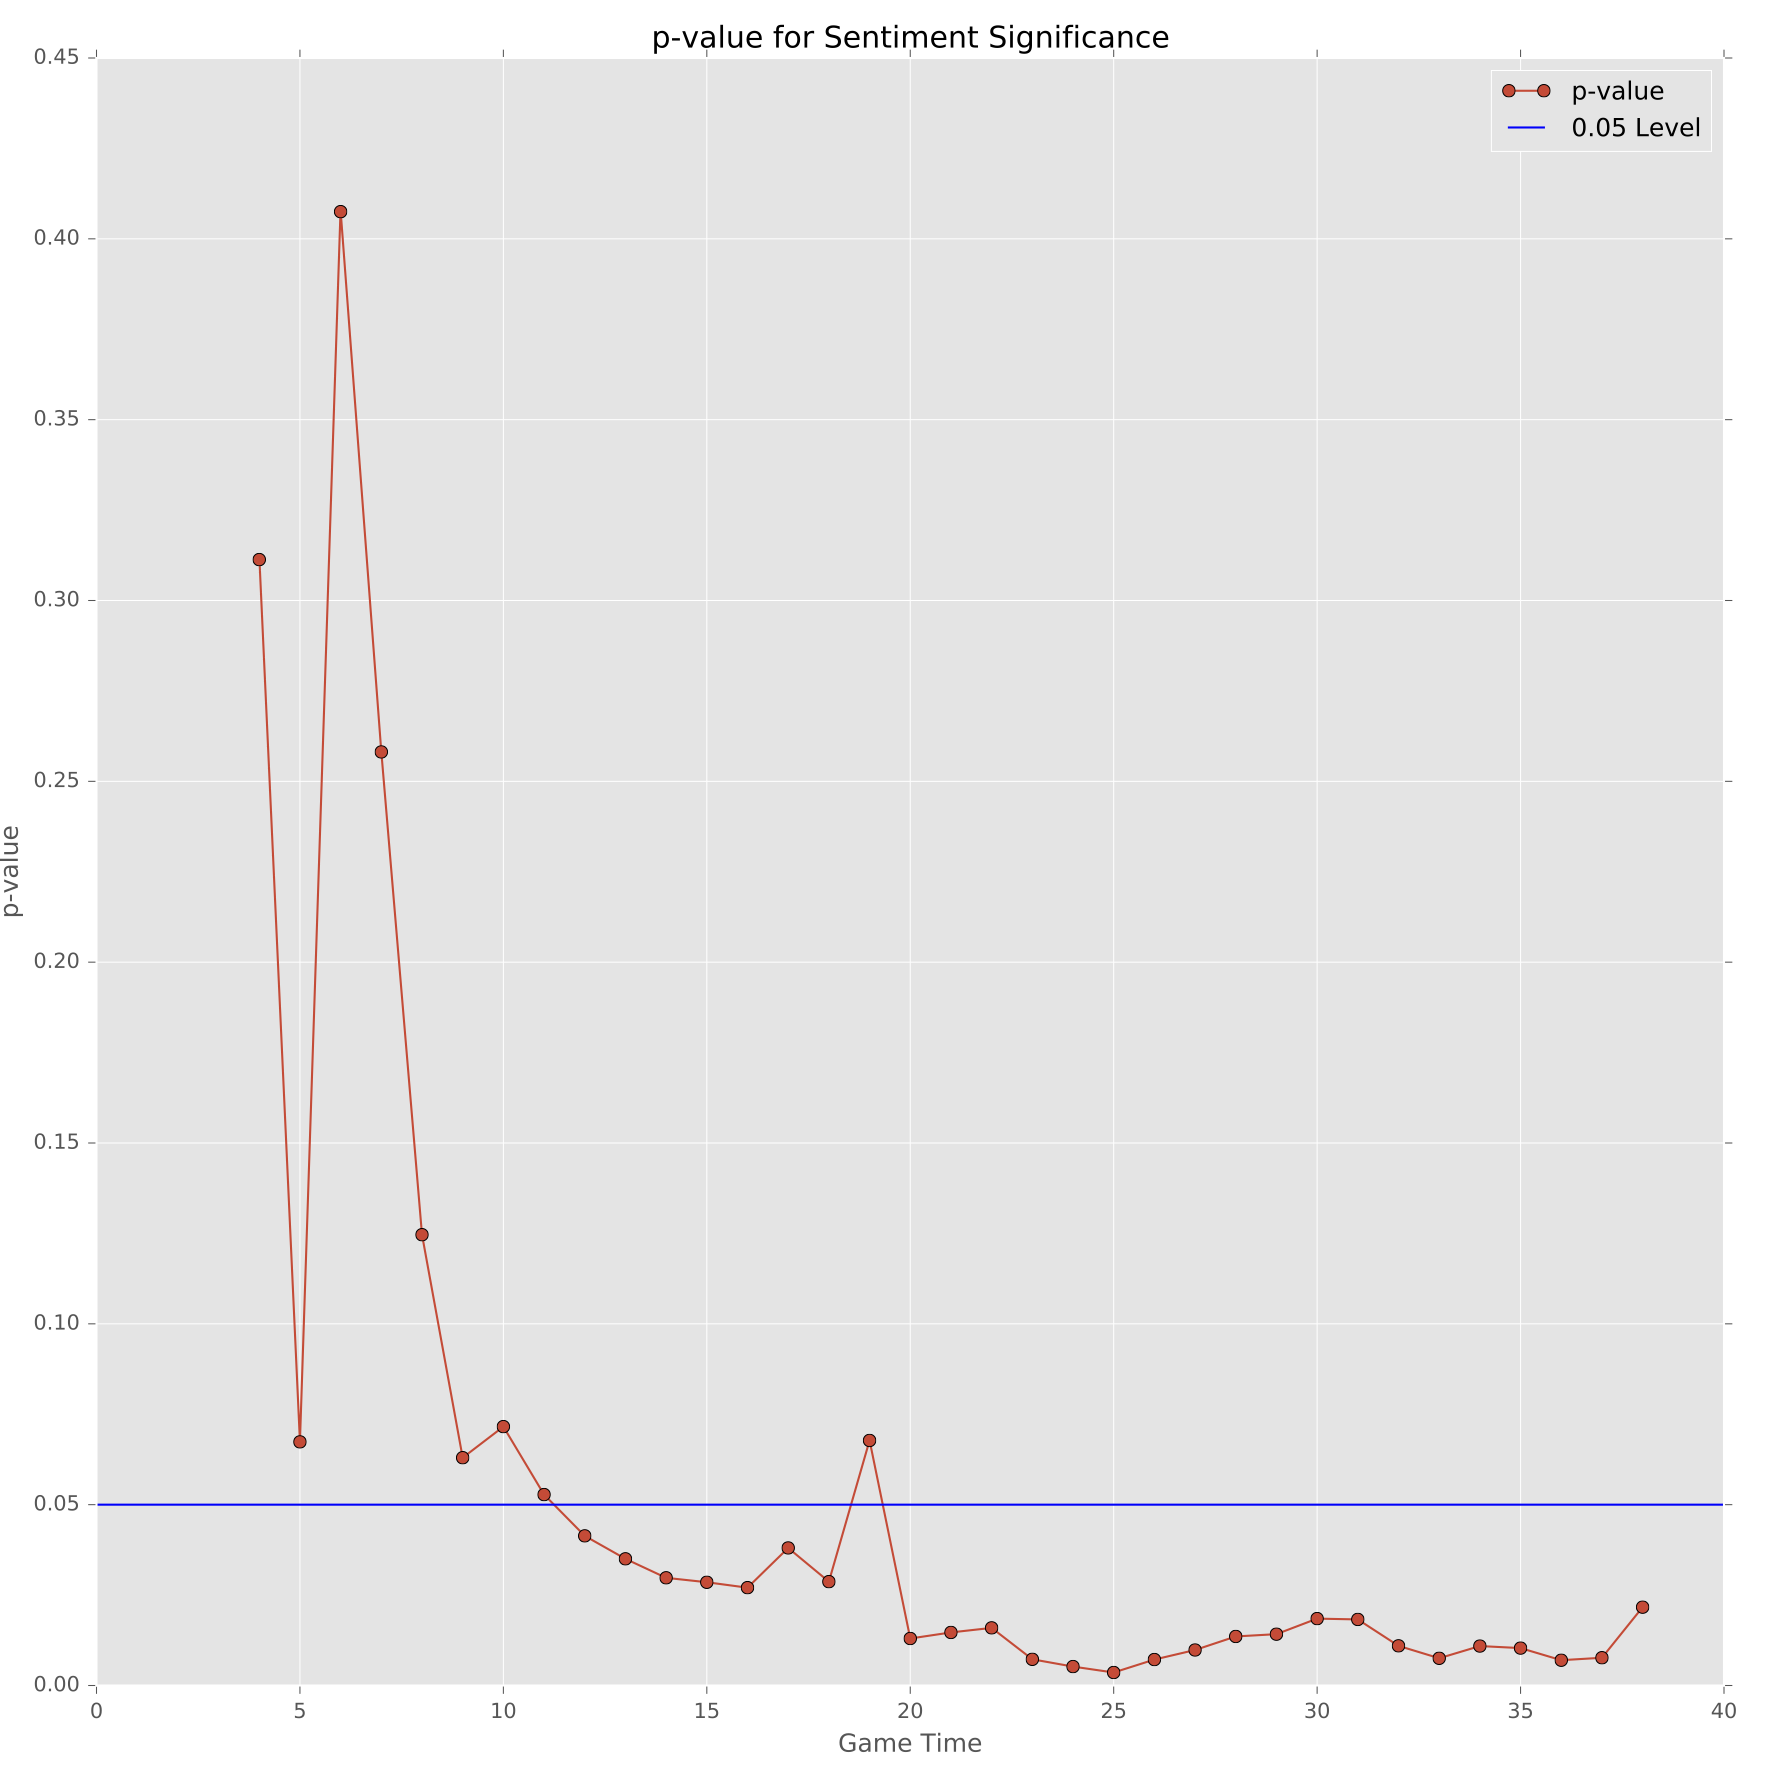
\includegraphics[scale = 0.4] {Images/pValuePlot.png} 
	\caption{Predictive power of sentiment difference over time}\label{fig:significance}
\end{figure}

To create Figure \ref{fig:significance} above, we ran logistic regressions for the winner of the game with varying amounts of time remaining. We found that the total sentiment difference between the two teams only started being consistently significant at the 0.05 percent level in the second half, where it was an important predictor of the final outcome. We can see from the graph that in the early stages of the game, Twitter's opinion about a team is not nearly as effective at predicting the final outcome. 

From this, we can infer that Twitter does have some predictive power to evaluate the winner of each game from an intermediate stage. To properly assess this, we compare the standard in-game prediction models to those that utilize Twitter sentiment. The canonical mid-game models consist of logistic regressions that use just two variables: the current margin and an ex ante predictor of team quality (typically the betting line provided by Vegas before the game). This was the basis of the models that FiveThirtyEight popularized during the 2016 tournament while creating their in-game prediction models. 

%% Image 8: Twitter-based models compared to general models
\begin{figure} [H]
	\centering
	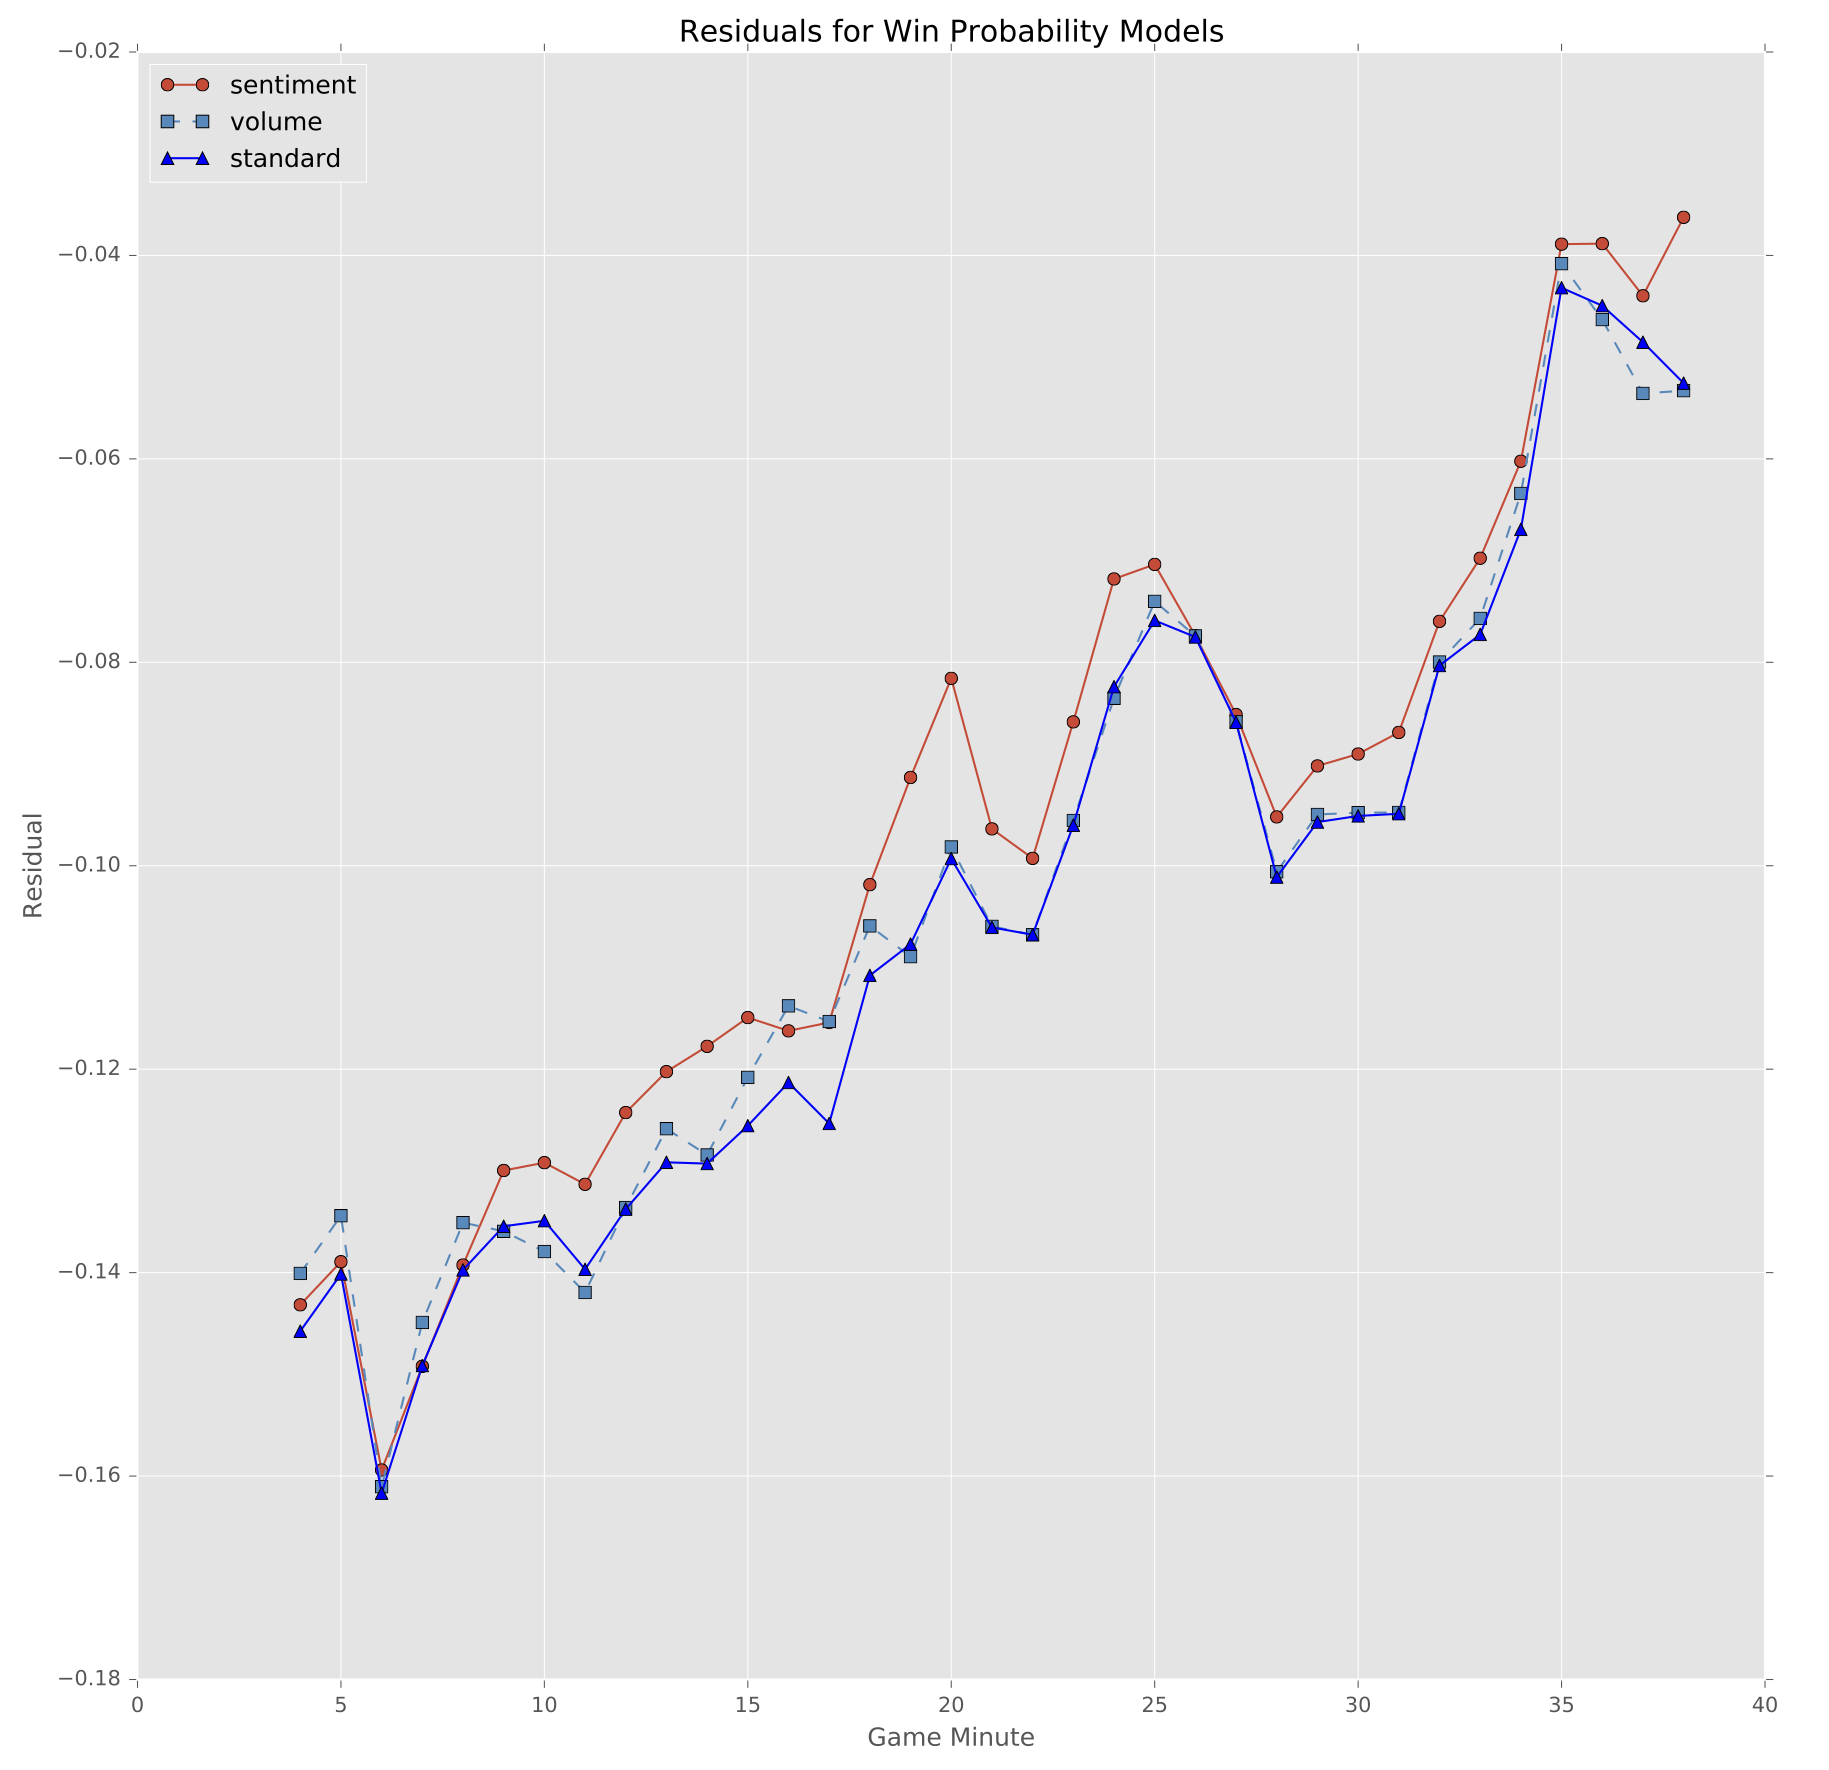
\includegraphics[scale = 0.4] {Images/VolumeSentResidualPlot.png} 
	\caption{Relative quality of standard and updated models at each minute of the game}\label{fig:modelcomparison}
\end{figure}

In Figure \ref{fig:modelcomparison} above, we look at how the standard model measures against the logistic regression model that includes Twitter sentiment and Twitter volume as explanatory factors. As can be inferred from the above graph, a logistic regression model that adds in Twitter sentiment outperforms the standard model at every point in the game---the residual for the updated model is consistently smaller than the residual for the standard model. We note that these results do appear to reinforce a result we first saw in Table 5, which indicates that Twitter sentiment carries more predictive power than Twitter volume.\footnote{Recall that in section 4.1 we had shown that Twitter volume is more responsive to past events, however.}

These results provide more substantial evidence for what we had inferred before: Twitter captures important predictive information that previous models did not. Table 9 shows the results of global regressions that merely confirm the relevance of both Twitter sentiment and volume. In Columns (2), (3), and (4) the two metrics are statistically significant at the 0.01 percent significance level and carry positive coefficients, implying that the higher Twitter is on a team, the more likely they are to eventually come out victorious. 

\section*{Regression Tables}

%% Table 1: How Twitter Responds to Changes in Margin (Sentiment)
\begin{table}[H] 
\centering 
\caption{Twitter Responsiveness to Game Events (pt. 1)}\label{table:sentresponsiveness} 
\begin{tabular*}{\textwidth}{@{\extracolsep{\fill}}lccc} 
\hline 
\hline
 & \multicolumn{3}{c}{\textit{Dependent variable:}} \\ 
\cline{2-4} 
\\[-3.0ex] & \multicolumn{3}{c}{SentDiff\_Period} \\ 
\\[-1.5ex] & (1) & (2) & (3)\\ 
\hline
 Margin\_Period\_Lag1 & 0.891$^{**}$ & 0.881$^{**}$ & 0.910$^{**}$ \\ 
  & (0.367) & (0.366) & (0.370) \\ 
 Margin\_Period\_Lag2 &  &  & 0.864$^{**}$ \\ 
  &  &  & (0.377) \\ 
 Vegas\_Line &  & $-$1.008$^{***}$ & $-$0.973$^{***}$ \\ 
  &  & (0.231) & (0.237) \\ 
 QualityDiff &  & 35.390$^{***}$ & 32.811$^{***}$ \\ 
  &  & (10.041) & (10.304) \\ 
 TwitterDiff &  & $-$0.004 & $-$0.006 \\ 
  &  & (0.011) & (0.011) \\ 
 Min\_End &  & 0.068 & 0.061 \\ 
  &  & (0.075) & (0.079) \\ 
\hline \\[-1.8ex] 
Observations & 1,306 & 1,306 & 1,266 \\ 
R$^{2}$ & 0.005 & 0.021 & 0.023 \\ 
Adjusted R$^{2}$ & 0.004 & 0.017 & 0.018 \\ 
Residual Std. Error & 30.443 & 30.238 & 30.562 \\ 
F Statistic & 5.897$^{**}$ & 5.548$^{***}$ & 4.972$^{***}$ \\ 
\hline 
\hline \\[-1.8ex] 
\end{tabular*} 
\end{table} 

%% Table 2: How Twitter Responds to Changes in Margin (Volume)
\begin{table}[H] 
\centering 
\caption{Twitter Responsiveness to Game Events (pt. 2)} 
\label{table:volumeresponsiveness} 
\begin{tabular*}{\textwidth}{@{\extracolsep{\fill}}lccc} 
\hline 
\hline
 & \multicolumn{3}{c}{\textit{Dependent variable:}} \\ 
\cline{2-4} 
\\[-3.0ex] & \multicolumn{3}{c}{VolDiff\_Period} \\ 
\\[-1.5ex] & (1) & (2) & (3)\\ 
\hline
 Margin\_Period\_Lag1 & 6.253$^{***}$ & 5.877$^{***}$ & 6.028$^{***}$ \\ 
  & (1.259) & (1.237) & (1.246) \\ 
 Margin\_Period\_Lag2 &  &  & 4.779$^{***}$ \\ 
  &  &  & (1.268) \\ 
 Vegas\_Line &  & $-$1.454$^{*}$ & $-$1.416$^{*}$ \\ 
  &  & (0.781) & (0.797) \\ 
 QualityDiff &  & 129.964$^{***}$ & 122.143$^{***}$ \\ 
  &  & (33.914) & (34.662) \\ 
 TwitterDiff &  & 0.165$^{***}$ & 0.168$^{***}$ \\ 
  &  & (0.036) & (0.037) \\ 
 Min\_End &  & $-$0.630$^{**}$ & $-$0.679$^{**}$ \\ 
  &  & (0.253) & (0.267) \\ 
\hline \\[-1.8ex] 
Observations & 1,306 & 1,306 & 1,266 \\ 
R$^{2}$ & 0.019 & 0.063 & 0.073 \\ 
Adjusted R$^{2}$ & 0.018 & 0.060 & 0.069 \\ 
Residual Std. Error & 104.377 & 102.132 & 102.812 \\ 
F Statistic & 24.685$^{***}$  & 17.550$^{***}$ & 16.599$^{***}$ \\
\hline 
\hline \\[-1.8ex] 
\end{tabular*} 
\end{table} 

%% Table 3: Twitter Sensitivity to Game Events During Closing Minutes
\begin{table}[H] 
\centering 
\caption{Twitter Responsiveness to Game Events (Closing Minutes)} 
\label{table:endgamesensitivity} 
\begin{tabular*}{\textwidth}{@{\extracolsep{\fill}}lcccc} 
\hline 
\hline
 & \multicolumn{4}{c}{\textit{Dependent variable:}} \\ 
\cline{2-5} 
\\[-3.0ex] & \multicolumn{2}{c}{SentDiff\_Period} & \multicolumn{2}{c}{VolDiff\_Period} \\ 
\\[-1.5ex] & (1) & (2) & (3) & (4)\\ 
\hline
 Margin\_Period & 3.080$^{***}$ &  & 9.598$^{***}$ &  \\ 
  & (0.898) &  & (2.980) &  \\ 
 Margin\_Period\_Lag1 &  & 1.325 &  & 7.570$^{**}$ \\ 
  &  & (0.934) &  & (3.071) \\ 
 Vegas\_Line & $-$1.691$^{***}$ & $-$1.802$^{***}$ & 1.061 & 0.671 \\ 
  & (0.585) & (0.594) & (1.941) & (1.953) \\ 
 QualityDiff & 54.306$^{**}$ & 61.013$^{**}$ & 44.282 & 60.681 \\ 
  & (25.706) & (26.013) & (85.282) & (85.559) \\ 
 TwitterDiff & $-$0.012 & $-$0.012 & 0.451$^{***}$ & 0.447$^{***}$ \\ 
  & (0.028) & (0.028) & (0.092) & (0.092) \\ 
 Min\_End & $-$0.526 & $-$0.719 & $-$2.755 & $-$3.466 \\ 
  & (0.740) & (0.751) & (2.455) & (2.470) \\ 
\hline \\[-1.8ex] 
Observations & 316 & 316 & 316 & 316 \\ 
R$^{2}$ & 0.068 & 0.039 & 0.133 & 0.121 \\ 
Adjusted R$^{2}$ & 0.053 & 0.024 & 0.119 & 0.107 \\ 
Residual Std. Error & 37.840 & 38.427 & 125.537 & 126.387 \\ 
F Statistic & 4.535$^{***}$ & 2.520$^{**}$ & 9.490$^{***}$ & 8.531$^{***}$ \\ 
\hline 
\hline \\[-1.8ex] 
\end{tabular*} 
\end{table} 

%% Table 4: Can Twitter Sentiment Predict Future Margins
\begin{table}[H] 
\centering 
\caption{The Accuracy of the Crowds (pt. 1)} 
\label{table:accuracypart1} 
\begin{tabular*}{\textwidth}{@{\extracolsep{\fill}}lccc} 
\hline 
\hline
 & \multicolumn{3}{c}{\textit{Dependent variable:}} \\ 
\cline{2-4} 
\\[-3.0ex] & \multicolumn{3}{c}{Margin\_Period} \\ 
\\[-1.5ex] & (1) & (2) & (3)\\ 
\hline
 SentDiff\_Period\_Lag1 & 0.006$^{***}$ & 0.006$^{***}$ & 0.006$^{***}$ \\ 
  & (0.002) & (0.002) & (0.002) \\ 
 SentDiff\_Period\_Lag2 &  &  & 0.001 \\ 
  &  &  & (0.003) \\ 
 SentDiff\_Period\_Lag3 &  &  & $-$0.003 \\ 
  &  &  & (0.002) \\ 
 Vegas\_Line &  & 0.009 & 0.003 \\ 
  &  & (0.018) & (0.019) \\ 
 QualityDiff &  & 0.983 & 1.239 \\ 
  &  & (0.780) & (0.809) \\ 
 TwitterDiff &  & 0.0003 & 0.0002 \\ 
  &  & (0.001) & (0.001) \\ 
 Min\_End &  & 0.004 & 0.007 \\ 
  &  & (0.006) & (0.006) \\ 
\hline \\[-1.8ex] 
Observations & 1,306 & 1,306 & 1,226 \\ 
R$^{2}$ & 0.006 & 0.012 & 0.015 \\ 
Adjusted R$^{2}$ & 0.005 & 0.008 & 0.009 \\ 
Residual Std. Error & 2.342 & 2.338 & 2.344 \\ 
F Statistic & 7.250$^{***}$ & 3.106$^{***}$ & 2.638$^{**}$ \\ 
\hline 
\hline \\[-1.8ex] 
\end{tabular*} 
\end{table} 

%% Table 5:
\begin{table}[H] 
\centering 
\caption{The Accuracy of the Crowds (pt. 2)} 
\label{table:accuracypart2} 
\begin{tabular*}{\textwidth}{@{\extracolsep{\fill}}lcccc} 
\hline 
\hline
 & \multicolumn{4}{c}{\textit{Dependent variable:}} \\ 
\cline{2-5} 
\\[-3.0ex] & \multicolumn{4}{c}{Margin\_Period} \\ 
\\[-1.5ex] & (1) & (2) & (3) & (4)\\ 
\hline
  VolDiff\_Period\_Lag1 & 0.002$^{***}$ & 0.002$^{***}$ & 0.002$^{**}$ & 0.003$^{***}$ \\ 
  & (0.001) & (0.001) & (0.001) & (0.001) \\ 
 SentDiff\_Period\_Lag1 &  &  & 0.004 &  \\ 
  &  &  & (0.002) &  \\ 
 VolDiff\_Period\_Lag2 &  &  &  & 0.0004 \\ 
  &  &  &  & (0.001) \\ 
 VolDiff\_Period\_Lag3 &  &  &  & $-$0.002$^{**}$ \\ 
  &  &  &  & (0.001) \\ 
 Vegas\_Line &  & 0.006 & 0.009 & 0.0004 \\ 
  &  & (0.018) & (0.018) & (0.018) \\ 
 QualityDiff &  & 0.902 & 0.837 & 1.224 \\ 
  &  & (0.780) & (0.781) & (0.806) \\ 
 TwitterDiff &  & $-$0.00003 & 0.0001 & 0.00005 \\ 
  &  & (0.001) & (0.001) & (0.001) \\ 
 Min\_End &  & 0.005 & 0.005 & 0.008 \\ 
  &  & (0.006) & (0.006) & (0.006) \\ 
\hline \\[-1.8ex] 
Observations & 1,306 & 1,306 & 1,306 & 1,226 \\ 
R$^{2}$ & 0.009 & 0.014 & 0.016 & 0.021 \\ 
Adjusted R$^{2}$ & 0.008 & 0.010 & 0.011 & 0.015 \\ 
Residual Std. Error & 2.338 & 2.335 & 2.334 & 2.337 \\ 
F Statistic & 11.852$^{***}$ & 3.686$^{***}$ & 3.435$^{***}$ & 3.675$^{***}$  \\ 
\hline 
\hline \\[-1.8ex] 
\end{tabular*} 
\end{table} 

%% Table 6: Reversion to the Mean
\begin{table}[H] 
\centering 
\caption{Reversion to the Mean} 
\label{table:meanreversion} 
\begin{tabular*}{\textwidth}{@{\extracolsep{\fill}}lcccc} 
\hline 
\hline
 & \multicolumn{4}{c}{\textit{Dependent variable:}} \\ 
\cline{2-5} 
\\[-3.0ex] & \multicolumn{4}{c}{Margin\_Period} \\ 
\\[-1.5ex] & (1) & (2) & (3) & (4)\\ 
\hline
 Margin\_TOT\_Lag1 & $-$0.018$^{**}$ & $-$0.023$^{***}$ & $-$0.019$^{**}$ & $-$0.024$^{***}$ \\ 
  & (0.008) & (0.008) & (0.008) & (0.008) \\ 
 SentDiff\_Total\_Lag1 &  & 0.001$^{**}$ &  & 0.001$^{**}$ \\ 
  &  & (0.0004) &  & (0.0004) \\ 
 VolDiff\_Total\_Lag1 &  &  & 0.00004 & 0.00005 \\ 
  &  &  & (0.0001) & (0.0001) \\ 
 Vegas\_Line & 0.005 & 0.016 & 0.005 & 0.017 \\ 
  & (0.018) & (0.019) & (0.018) & (0.019) \\ 
 QualityDiff & 1.679$^{**}$ & 1.364$^{*}$ & 1.631$^{**}$ & 1.303 \\ 
  & (0.802) & (0.815) & (0.805) & (0.819) \\ 
 TwitterDiff & 0.0004 & 0.0005 & 0.0003 & 0.0003 \\ 
  & (0.001) & (0.001) & (0.001) & (0.001) \\ 
 Min\_End & 0.002 & 0.001 & 0.002 & 0.002 \\ 
  & (0.006) & (0.006) & (0.006) & (0.006) \\ 
\hline \\[-1.8ex] 
Observations & 1,306 & 1,306 & 1,306 & 1,306 \\ 
R$^{2}$ & 0.011 & 0.014 & 0.011 & 0.015 \\ 
Adjusted R$^{2}$ & 0.007 & 0.010 & 0.007 & 0.009 \\ 
Residual Std. Error & 2.339 & 2.336 & 2.340 & 2.337 \\ 
F Statistic & 2.865$^{**}$ & 3.111$^{***}$ & 2.454$^{**}$ & 2.744$^{***}$ \\ 
\hline 
\hline \\[-1.8ex] 
\end{tabular*} 
\end{table} 

%% Table 7: Generalized Linear Model
\begin{table}[H] 
\centering 
\caption{Logistic Regressions for Winner Prediction} 
\label{table:winnerprediction} 
\begin{tabular*}{\textwidth}{@{\extracolsep{\fill}}lcccc} 
\hline 
\hline
 & \multicolumn{4}{c}{\textit{Dependent variable:}} \\ 
\cline{2-5} 
\\[-3.0ex] & \multicolumn{4}{c}{Winner} \\ 
\\[-1.5ex] & (1) & (2) & (3) & (4)\\ 
\hline
 Vegas\_Line & $-$0.041$^{***}$ & $-$0.034$^{**}$ & $-$0.044$^{***}$ & $-$0.038$^{***}$ \\ 
  & (0.014) & (0.014) & (0.014) & (0.014) \\ 
 Margin\_TOT & 0.173$^{***}$ & 0.166$^{***}$ & 0.168$^{***}$ & 0.160$^{***}$ \\ 
  & (0.012) & (0.012) & (0.012) & (0.012) \\ 
 SentDiff\_Total &  & 0.001$^{***}$ &  & 0.001$^{***}$ \\ 
  &  & (0.0005) &  & (0.001) \\ 
 VolDiff\_Total &  &  & 0.0002$^{**}$ & 0.0002$^{**}$ \\ 
  &  &  & (0.0001) & (0.0001) \\ 
\hline \\[-1.8ex] 
Observations & 1,346 & 1,346 & 1,346 & 1,346 \\ 
Log Likelihood & $-$594.303 & $-$590.365 & $-$591.049 & $-$587.436 \\ 
Akaike Inf. Crit. & 1,194.606 & 1,188.730 & 1,190.097 & 1,184.873 \\
\hline 
\hline \\[-1.8ex] 
\end{tabular*} 
\end{table} 

\end{doublespacing}
\end{document}